\documentclass[Royal,times,sageh]{sagej}

\usepackage{moreverb,url,natbib, multirow, tabularx}
\usepackage[colorlinks,bookmarksopen,bookmarksnumbered,citecolor=red,urlcolor=red]{hyperref}



% tightlist command for lists without linebreak
\providecommand{\tightlist}{%
  \setlength{\itemsep}{0pt}\setlength{\parskip}{0pt}}



\let\pandocbounded\ignorespaces \renewcommand{\pandocbounded}[1]{#1}


\begin{document}


\setcitestyle{aysep={,}}

\title{COMPORTAMIENTO DE LA CARTERA DE MICROCREDITO EN UNA INSTITUCIÓN
FINANCIERA DE DESARROLLO DE LAS CIUDADES DE LA PAZ Y ORURO, CONSIDERANDO
LOS FACTORES ECONOMICOS DE LOS PERIODOS 2022 AL 2024 EN BOLIVIA (CASO
CIDRE IFD)}

\runninghead{Diago Rojas}

\author{Diago Erick Rojas Soto\affilnum{1}}

\affiliation{\affilnum{1}{Universidad Católica Boliviana San Pablo sede
``La Paz''}}

\corrauth{Diago Erick Rojas Soto, Carrera de Economía e Inteligencia de
Negocios, UCB, La Paz, Bolivia}


\begin{abstract}
El análisis de la cartera de microcréditos de la Institución Financiera
de Desarrollo CIDRE IFD en Bolivia, específicamente en las ciudades de
La Paz y Oruro, revela que al cierre de 2024, la institución manejaba
más de 118 millones de dólares y contaba con más de 25,000 clientes, con
una concentración del 98\% en microcréditos. Este estudio destaca la
importancia del microcrédito como herramienta de inclusión financiera y
su impacto en la estabilidad económica de los prestatarios, así como la
necesidad de identificar factores que afectan su comportamiento para
diseñar estrategias que fortalezcan su impacto y mitiguen riesgos. A
pesar de un crecimiento económico positivo post-pandemia, la economía
boliviana ha mostrado una tendencia decreciente, con un crecimiento del
6.11\% en 2022, pero solo 3.6\% en 2023 y 2.14\% proyectado para 2024.
La alta tasa de desempleo y el aumento del trabajo informal complican la
recuperación económica, lo que pone en riesgo la operación de
instituciones como CIDRE IFD. El análisis busca generar conocimientos
que contribuyan a estrategias más resilientes, asegurando la
sostenibilidad de la institución y maximizando su impacto en el sector
microempresarial boliviano.
\end{abstract}

\keywords{MicrocréditoInstituciones Financieras de DesarrolloEconomía en
BoliviaAnálisis Financiero}

\maketitle

\newpage

\subsection{\texorpdfstring{1.
\textbf{Introduccion:}}{1. Introduccion:}}\label{introduccion}

El microcrédito ha emergido como una herramienta fundamental para la
inclusión financiera en Bolivia, especialmente en un contexto donde las
instituciones financieras de desarrollo juegan un papel crucial en el
empoderamiento de sectores vulnerables. A medida que el país enfrenta
desafíos económicos, como el aumento del desempleo y la precarización
laboral, el acceso a microcréditos se convierte en un recurso vital para
fomentar la estabilidad económica de los prestatarios y promover el
desarrollo sostenible. Este estudio se centra en el comportamiento de la
cartera de microcréditos de la Institución Financiera de Desarrollo
CIDRE IFD en las ciudades de La Paz y Oruro, analizando su evolución en
relación con factores económicos entre 2022 y 2024, con el objetivo de
identificar estrategias que fortalezcan su impacto y mitiguen los
riesgos asociados.

\subsection{\texorpdfstring{2.
\textbf{Antecedentes:}}{2. Antecedentes:}}\label{antecedentes}

Las instituciones financieras de desarrollo (IFD) en Bolivia han jugado
un papel esencial en la inclusión financiera, acercando servicios y
productos financieros a los sectores más vulnerables de la sociedad.
Estas instituciones no solo contribuyen al empoderamiento económico de
individuos y comunidades, sino que también se convierten en motores para
el desarrollo local y la reducción de desigualdades. En este contexto,
CIDRE IFD se destaca como una entidad comprometida con el fomento del
acceso al microcrédito, permitiendo a pequeños productores,
emprendedores y familias contar con el financiamiento necesario para
llevar a cabo sus proyectos y mejorar sus condiciones de vida. Sin
embargo, la gestión de la cartera de microcrédito no está exenta de
desafíos. CIDRE IFD ha enfrentado fluctuaciones económicas y contextos
complejos en las ciudades de La Paz y Oruro, regiones donde opera con
gran intensidad. Este estudio busca analizar los factores económicos que
han influido en el comportamiento de esta cartera entre 2022 y 2024. Al
comprender estas dinámicas, se espera aportar recomendaciones prácticas
para mejorar la resiliencia de CIDRE IFD y potenciar su impacto en la
promoción de la inclusión financiera en Bolivia.

\subsection{\texorpdfstring{3.
\textbf{Motivacion:}}{3. Motivacion:}}\label{motivacion}

Para una Institución Financiera de Desarrollo como CIDRE (estudio de
caso) la cartera de préstamos se constituye en la proporción más
importante del activo y, por tanto, la principal fuente de sus ingresos.
Pero cuando el entorno económico y social de un pais en este caso en
Bolivia presenta cambios que inciden en la economía de la población
económicamente activa, sin duda, puede incidir negativamente en el
comportamiento regular de la cartera

El analizar la data del negocio principal de una Institución Financiera
de Desarrollo como es el estudio de caso CIDRE IFD me permite determinar
la incidencia de la economía en Bolivia en un negocio que aporta al
desarrollo de las unidades económicas microempresariales de las ciudades
de La Paz y Oruro.

\subsection{\texorpdfstring{4. \textbf{Pregunta de
investigación:}}{4. Pregunta de investigación:}}\label{pregunta-de-investigaciuxf3n}

¿Cuál es la incidencia de los factores económicos de los periodos 2022
al 2024 en Bolivia, en el comportamiento de la cartera de microcrédito
en una Institución Financiera de Desarrollo de las ciudades de La Paz y
Oruro? (caso CIDRE IFD)

\subsection{\texorpdfstring{5.
\textbf{Objetivos:}}{5. Objetivos:}}\label{objetivos}

\textbf{4.1. Objetivo General:}

Analizar la incidencia de los factores económicos en el comportamiento
de la cartera de microcréditos de CIDRE IFD en las ciudades de La Paz y
Oruro durante los periodos 2022-2024.

\textbf{4.2. Objetivos Específicos:}

- Evaluar el impacto de las fluctuaciones macroeconómicas bolivianas en
la cartera de microcréditos

\begin{itemize}
\item
  Identificar la relación entre el empleo informal y la morosidad
  crediticia
\item
  Proponer estrategias de gestión de cartera adaptadas al contexto
  económico boliviano
\end{itemize}

Motivación Para una Institución Financiera de Desarrollo como CIDRE IFD,
la cartera de préstamos constituye no solo el mayor activo, sino también
la principal fuente de ingresos. La estabilidad y buen desempeño de esta
cartera son esenciales para asegurar la sostenibilidad financiera de la
institución y, por ende, su capacidad para promover la inclusión
financiera. Sin embargo, los cambios en el entorno económico y social,
como los experimentados en Bolivia entre 2022 y 2024, pueden afectar
significativamente el comportamiento regular de esta cartera,
especialmente en la economía de la población activa, poniendo en riesgo
tanto la recuperación de los préstamos como la operación general de la
institución.

Analizar la data relacionada con el negocio principal de CIDRE IFD
permite identificar cómo los factores económicos de estos años
impactaron en las microempresas de La Paz y Oruro, regiones clave para
el desarrollo económico local. Este análisis no solo busca entender
estas dinámicas, sino también generar conocimientos que contribuyan al
diseño de estrategias más resilientes, asegurando la sostenibilidad de
la institución y maximizando su impacto en el fortalecimiento del sector
microempresarial boliviano.

\subsection{\texorpdfstring{6. \textbf{Revision de la
literatura:}}{6. Revision de la literatura:}}\label{revision-de-la-literatura}

\textbf{6.1 La economía en Bolivia: Un análisis crítico post-pandemia
2022-2024}

De acuerdo con el ``Informe del Milenio sobre la economía en Bolivia''
(2023-2024), tras la pandemia del COVID-19, la economía boliviana mostró
una tendencia positiva con un crecimiento del 6.11\% en 2022. Sin
embargo, este crecimiento se desaceleró a 3.6\% en 2023, y para 2024 el
INE publicó un crecimiento de solo 2.14\%. Esta tendencia decreciente
refleja una crisis inminente manifestada por la escasez de divisas y
combustibles, agudizando ``\ldots los desequilibrios fiscales,
monetarios, cambiarios y financieros, que conllevan riesgos para la
estabilidad macroeconómica'' (Informe Nuevo Milenio, 2024, pág. 7).

\begin{figure}

{\centering 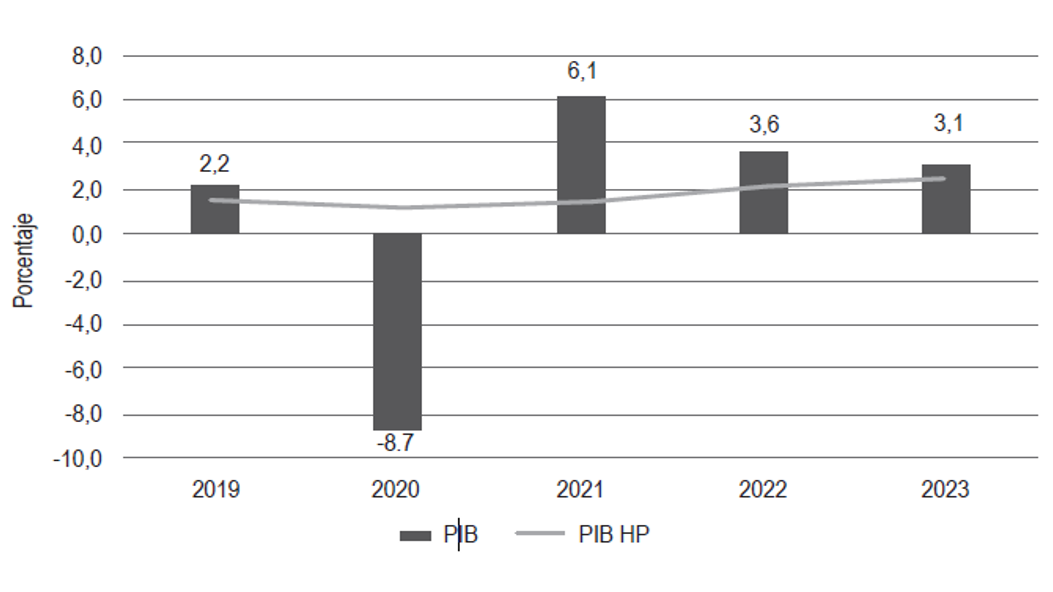
\includegraphics[width=1\linewidth]{Imagen 1} 

}

\caption{Crecimiento trimestral del PIB en 2022 y 2023 (variación porcentual)}\label{fig:i1}
\end{figure}

Otro factor que amerita una valoración en medida que condice con el tema
de investigación propuesto, es analizar el mercado laboral en nuestro
país, de acuerdo al ``Informe del Milenio sobre la economía en Bolivia''
2023 y 2024, exponen que la tasa de desempleo es alta y que es producto
de un problema que deviene del denominado ``precarización'' manifestado
en el increíble crecimiento del ``cuentapropismo''; un tipo de trabajo
predominantemente informal, desamparada y casi siempre mal remunerada y
con propensión a predominar. el 70\% de los hogares urbanos del país se
encuentran en situación de ocupación informal (gráfico No 2). El aumento
de la actividad ``informal'' está demostrando que las oportunidades de
un empleo formal son menores y que la opción para generar ingresos se
concentra en la formación de economías alternas, a través de actividades
diversas, sobre todo de comercio, servicio, etc.

Gráfico No 2 \textbf{Hogares según mercado laboral (en porcentaje, sobre
el total de la población urbana)}

\begin{figure}

{\centering 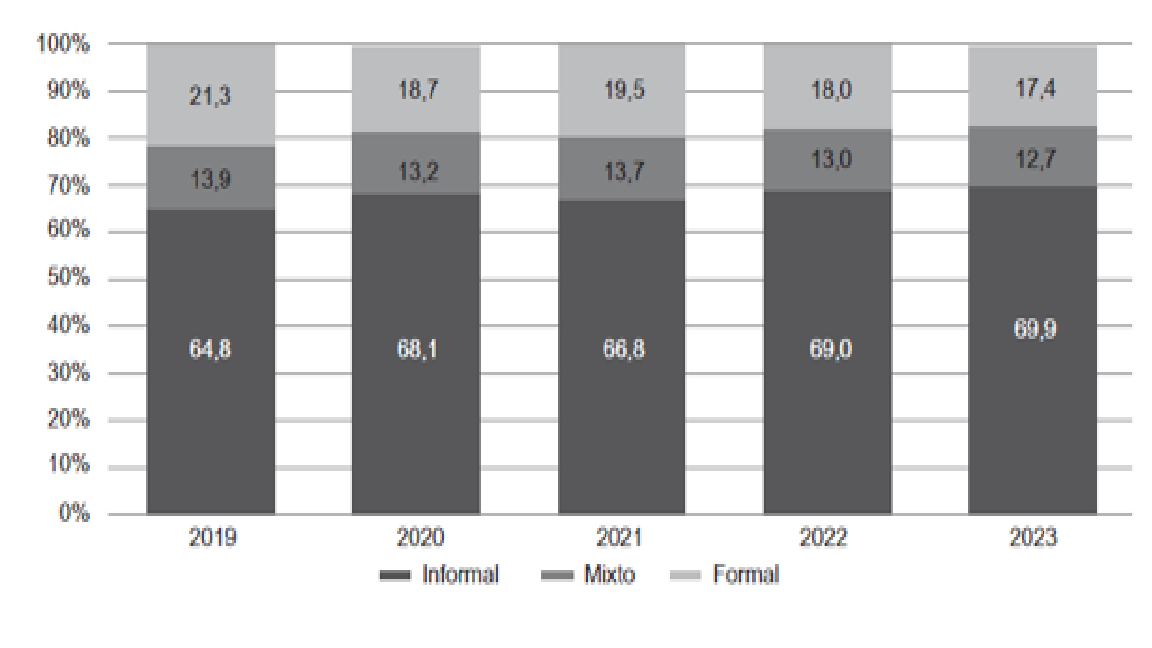
\includegraphics[width=0.8\linewidth]{Imagen 2} 

}

\caption{Hogares según mercado laboral (en porcentaje, sobre el total de la población urbana)}\label{fig:i2}
\end{figure}

Fuente: ``Informe del Milenio sobre la economía en Bolivia'' 2024

En Bolivia, las microempresas representan un segmento importante del
mercado, especialmente en las ciudades capitales. Aunque muchas operan
de manera informal y generan ingresos limitados, son fundamentales para
el ecosistema financiero, en particular el sector de microfinanzas.

Según la Fundación ARU y el Ministerio de Desarrollo Productivo y
Economía Plural (MDPyEP), las micro y pequeñas empresas (MyPE) se
identifican por tres criterios: \textbf{ventas anuales, patrimonio y
número de empleados}. La OIT establece que una microempresa tiene entre
\textbf{2 y 9 empleados}, mientras que una pequeña cuenta con \textbf{10
a 49}. El INE maneja distintos rangos según el sector económico: en
manufactura, una microempresa tiene \textbf{hasta 10 empleados} y una
pequeña hasta \textbf{30}; en comercio y servicios, una microempresa
opera con \textbf{hasta 5 empleados} y una pequeña con \textbf{hasta
20}.

Las microempresas requieren financiamiento para su crecimiento, pero
enfrentan barreras de acceso al crédito debido a factores externos (como
condiciones de mercado) e internos (como la falta de información
financiera adecuada). Esto genera \textbf{exclusión financiera},
dificultando su desarrollo y sostenibilidad económica.

\textbf{6.2 LAS MICROFINANZAS: ENFOQUE HACIA SECTORES INFORMALES (MICRO
Y PEQUEÑAS EMPRESA.}

Un artículo publicado en ABC Economía (2024) exploró el comportamiento
de la cartera de créditos en Bolivia y su relación con el microcrédito.
El estudio señala que, a lo largo de las últimas décadas, la expansión
del microcrédito ha desempeñado un papel crucial en la inclusión
financiera de sectores tradicionalmente marginados. Sin embargo, también
destaca los desafíos asociados, como el riesgo de morosidad y la
necesidad de diseñar políticas adecuadas para garantizar la
sostenibilidad del sector financiero. Utilizando datos recientes, el
artículo analiza la evolución del microcrédito en relación con la
estabilidad macroeconómica del país.

Un estudio de la Fundación ARU (2024) evaluó el impacto del microcrédito
en Bolivia, con evidencia del crédito productivo individual otorgado por
el Banco de Desarrollo Productivo (BDP). Los investigadores encontraron
que el acceso al microcrédito ha impulsado el crecimiento de pequeños
emprendimientos, mejorando sus ingresos y estabilidad económica. Sin
embargo, el estudio también señala que el efecto del crédito varía
dependiendo de la estructura del negocio y la capacitación financiera
del prestatario. Además, se destaca que los programas de financiamiento
deben estar acompañados de asistencia técnica para maximizar su impacto
en la productividad y sostenibilidad de los emprendimientos.

El estudio del microcrédito en Bolivia permite comprender su papel como
una herramienta de inclusión financiera y su influencia en la
estabilidad económica de los prestatarios. Identificar los factores que
afectan el comportamiento de la cartera de microcréditos es crucial para
diseñar estrategias que fortalezcan su impacto y mitiguen riesgos
asociados, promoviendo así un desarrollo financiero más equitativo y
sostenible.

\subsection{\texorpdfstring{7 \textbf{Descripcion de los
datos:}}{7 Descripcion de los datos:}}\label{descripcion-de-los-datos}

El presente estudio utiliza un subconjunto de datos extraído de la base
de cartera de créditos de una entidad financiera. Este subconjunto se
compone de variables que permiten describir las características básicas
del cliente y las condiciones del crédito otorgado. En cuanto al perfil
del cliente, se consideran las variables edad, sexo y sector geográfico
(rural o urbano). Estas permiten analizar diferencias de comportamiento
crediticio según género, grupo etario y ubicación. Por otro lado, en el
ámbito crediticio, se seleccionan variables clave como el monto del
crédito, la tasa de interés aplicada, los días en mora (como indicador
de incumplimiento) y la calificación crediticia. Estas variables
permitirán explorar patrones asociados al riesgo de incumplimiento y
construir modelos predictivos en el marco de la minería de datos.

Variables de caracterización del cliente: - Edad - Sexo - Sector
geográfico: urbano o rural Variables crediticias: - Monto aprobado del
crédito - Tasa de interés - Días en mora - Calificación crediticia (A,
B, C, D, E)

\subsection{\texorpdfstring{\textbf{8. Justificación del Dataset
Nacional}}{8. Justificación del Dataset Nacional}}\label{justificaciuxf3n-del-dataset-nacional}

El dataset sobre la cartera de microcréditos de CIDRE IFD en La Paz y
Oruro se justifica dentro del contexto de una problemática clave en
Bolivia: la \textbf{inclusión financiera} y la \textbf{sostenibilidad de
las microempresas} frente a la desaceleración económica.

\textbf{Conexión con la Problemática Local}

La economía boliviana ha mostrado una tendencia decreciente desde 2022,
con una reducción en el crecimiento del PIB y un aumento en la
informalidad laboral. En este escenario, las \textbf{microempresas} y
los \textbf{emprendedores} enfrentan barreras estructurales para acceder
a financiamiento, lo que puede afectar directamente la estabilidad del
sistema financiero de desarrollo.

El dataset proporciona datos sobre clientes y su comportamiento
crediticio, lo que permite:

\begin{enumerate}
\def\labelenumi{\arabic{enumi}.}
\item
  \textbf{Identificar patrones de acceso al crédito}, diferenciando
  entre sectores urbanos y rurales.
\item
  \textbf{Evaluar el impacto de la economía nacional} en la capacidad de
  pago y tasas de mora.
\item
  \textbf{Analizar la calificación crediticia} para entender los riesgos
  y diseñar estrategias de mitigación.
\item
  \textbf{Optimizar la asignación de recursos} dentro de CIDRE IFD,
  ajustando políticas de financiamiento a las necesidades reales de los
  prestatarios.
\end{enumerate}

\subsection{\texorpdfstring{9. \textbf{Metodologia
aplicada:}}{9. Metodologia aplicada:}}\label{metodologia-aplicada}

Metodología Esta investigación adopta un enfoque cuantitativo y
predictivo, apoyado en técnicas de minería de datos, particularmente
modelos de regresión, con el fin de analizar el comportamiento de la
cartera de microcréditos de una Institución Financiera de Desarrollo
(CIDRE IFD) en las ciudades de La Paz y Oruro durante los años 2022 al
2024.

\begin{enumerate}
\def\labelenumi{\arabic{enumi}.}
\tightlist
\item
  Base de datos y variables La información utilizada proviene de la base
  de datos interna de CIDRE IFD, la cual contiene registros de
  operaciones crediticias en las regiones mencionadas. A partir de este
  conjunto amplio de variables, se seleccionaron las siguientes:
\end{enumerate}

Variables sociodemográficas:

Edad: variable cuantitativa continua.

Sexo: variable cualitativa binaria.

Sector rural/urbano: variable binaria.

Variables crediticias:

Monto aprobado: monto del crédito otorgado (cuantitativa).

Tasa de interés: tasa aplicada al crédito (cuantitativa).

Días en mora: número de días de incumplimiento en el pago
(cuantitativa).

Calificación crediticia: clasificación del cliente según su
comportamiento de pago (ordinal/categórica).

\begin{enumerate}
\def\labelenumi{\arabic{enumi}.}
\setcounter{enumi}{1}
\tightlist
\item
  Enfoque metodológico El análisis sigue la estructura planteada en el
  curso de regresión:
\end{enumerate}

Paso 1: Preparación de los datos Limpieza de registros con valores
faltantes o inconsistentes.

Transformación de variables categóricas en factores (por ejemplo, sexo y
sector).

Generación de variables derivadas si es necesario (como categorías de
edad o rangos de monto).

Paso 2: Relación de interés La variable dependiente principal es:

Días en mora, medida como una variable continua.

Se busca evaluar cómo las variables demográficas y crediticias influyen
en esta.

Paso 3: Modelo de regresión Se define el siguiente modelo general: \[
\text{DiasMora}_i = \beta_0 + \beta_1 \cdot \text{Edad}_i + \beta_2 \cdot \text{Sexo}_i + \beta_3 \cdot \text{Sector}_i + \beta_4 \cdot \text{Monto}_i + \beta_5 \cdot \text{TasaInteres}_i + \beta_6 \cdot \text{Calificación}_i + \epsilon_i
\]

En una segunda etapa, se evalúa también una versión log-transformada de
los días en mora si la distribución resulta altamente sesgada.

\begin{verbatim}
## [1] "C:/Users/Pavilion 15/Documents/ProyectoMineria2/Mineria2"
\end{verbatim}

\begin{verbatim}
##       Edad      Sexo     Sector        Monto              Tasa      
##  Min.   :19.0   F:6226   R:10523   Min.   :   3000   Min.   : 0.00  
##  1st Qu.:30.0   M:9313   U: 5016   1st Qu.:  28000   1st Qu.:11.50  
##  Median :38.0   N:   0             Median :  35000   Median :19.50  
##  Mean   :39.9                      Mean   :  45926   Mean   :17.39  
##  3rd Qu.:49.0                      3rd Qu.:  35100   3rd Qu.:21.00  
##  Max.   :81.0                      Max.   :1303500   Max.   :26.00  
##     DiasMora       Calificacion
##  Min.   :   0.00   A:14524     
##  1st Qu.:   0.00   B:  579     
##  Median :   0.00   C:  120     
##  Mean   :  18.65   D:   59     
##  3rd Qu.:   0.00   E:   39     
##  Max.   :3270.00   F:  218
\end{verbatim}

\begin{verbatim}
## 
## Call:
## lm(formula = log1p(DiasMora) ~ Edad + Sexo + Sector + Monto + 
##     Tasa + Calificacion, data = bd_total)
## 
## Residuals:
##     Min      1Q  Median      3Q     Max 
## -4.4894 -0.0688 -0.0625 -0.0396  4.0378 
## 
## Coefficients:
##                 Estimate Std. Error t value Pr(>|t|)    
## (Intercept)   -4.184e-03  1.959e-02  -0.214 0.830852    
## Edad           1.967e-04  3.150e-04   0.624 0.532425    
## SexoM         -3.213e-03  7.829e-03  -0.410 0.681521    
## SectorU       -3.910e-03  8.748e-03  -0.447 0.654965    
## Monto          1.849e-07  6.623e-08   2.792 0.005242 ** 
## Tasa           2.867e-03  8.324e-04   3.444 0.000575 ***
## CalificacionB  2.647e+00  2.007e-02 131.858  < 2e-16 ***
## CalificacionC  3.679e+00  4.323e-02  85.096  < 2e-16 ***
## CalificacionD  4.001e+00  6.153e-02  65.021  < 2e-16 ***
## CalificacionE  4.406e+00  7.562e-02  58.268  < 2e-16 ***
## CalificacionF  6.488e+00  3.238e-02 200.366  < 2e-16 ***
## ---
## Signif. codes:  0 '***' 0.001 '**' 0.01 '*' 0.05 '.' 0.1 ' ' 1
## 
## Residual standard error: 0.4715 on 15528 degrees of freedom
## Multiple R-squared:  0.8195, Adjusted R-squared:  0.8194 
## F-statistic:  7049 on 10 and 15528 DF,  p-value: < 2.2e-16
\end{verbatim}

El modelo de regresión ajustado busca evaluar los determinantes de los
días en mora de los clientes de CIDRE IFD, considerando una
transformación logarítmica para estabilizar la variabilidad de la
variable dependiente. Los resultados se presentan en términos de
coeficientes estimados, significancia estadística y capacidad
explicativa del modelo.

\textbf{1. Calidad y Significancia del Modelo} El coeficiente de
determinación ajustado (R² = 0.8194) indica que aproximadamente 82\% de
la variabilidad en los días de mora puede ser explicada por las
variables independientes incluidas en el análisis. Este nivel sugiere
una relación robusta entre las características crediticias y el
comportamiento de pago.

-\textbf{El estadístico F} (7049, p \textless{} 2.2e-16) confirma la
alta significancia del modelo en su conjunto, lo que implica que al
menos una de las variables explicativas tiene un efecto significativo
sobre la mora.

\textbf{Interpretación de los Coeficientes} Los coeficientes de
regresión reflejan el impacto relativo de cada variable sobre la
cantidad de días en mora.

\textbf{-Edad} (p = 0.532): No se identifica un efecto estadísticamente
significativo de la edad del cliente sobre la mora.

\textbf{-Sexo} (p = 0.681): La variable no muestra significancia, lo que
sugiere que no existen diferencias sistemáticas entre hombres y mujeres
respecto a su comportamiento de pago.

\textbf{-Sector geográfico} (p = 0.654): No se evidencia una relación
estadística entre la localización del prestatario (urbano/rural) y los
días en mora.

\textbf{Por otro lado, las siguientes variables presentan efectos
significativos en la probabilidad de mora:}

\textbf{Monto aprobado del crédito} (p = 0.005): Aunque su coeficiente
es pequeño (1.849e-07), indica que montos de crédito más elevados pueden
estar asociados con un ligero aumento en los días de mora.

\textbf{Tasa de interés} (p = 0.000575): Un coeficiente positivo
(2.867e-03) sugiere que tasas más altas incrementan los días en mora,
reflejando la carga financiera adicional que enfrentan los prestatarios
con créditos más costosos.

\textbf{Impacto de la Calificación Crediticia} La variable calificación
crediticia es la que presenta un mayor efecto sobre la mora.

Clientes con calificación A sirven como grupo de referencia.

Clientes con calificación B, C, D, E y F muestran coeficientes
crecientes, lo que indica que, a medida que disminuye la calificación,
se incrementan significativamente los días en mora.

Calificación F (coeficiente = 6.488, p \textless{} 2e-16) presenta la
mayor incidencia en mora, lo que refleja un alto riesgo de
incumplimiento en este segmento.

\begin{figure}

{\centering 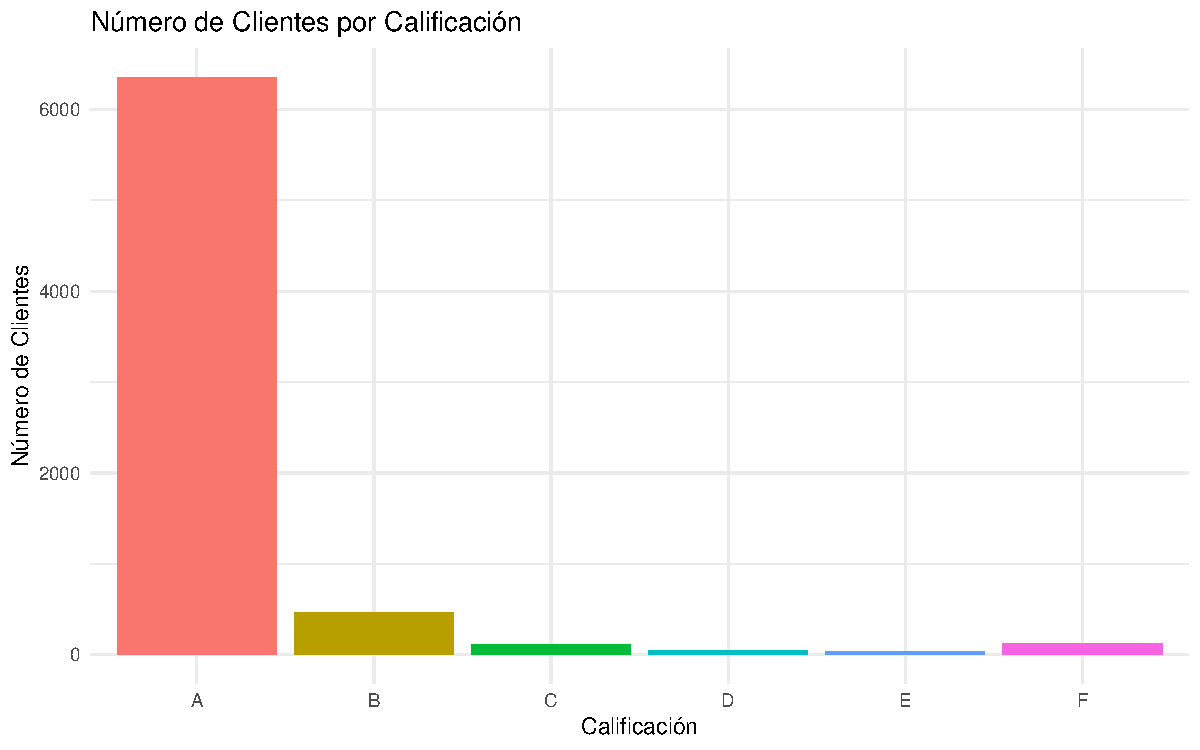
\includegraphics[width=0.9\linewidth]{Mineria2_files/figure-latex/graficos_ajustados-1} 

}

\caption{Número de Clientes por Calificación}\label{fig:graficos_ajustados-1}
\end{figure}
\begin{figure}

{\centering 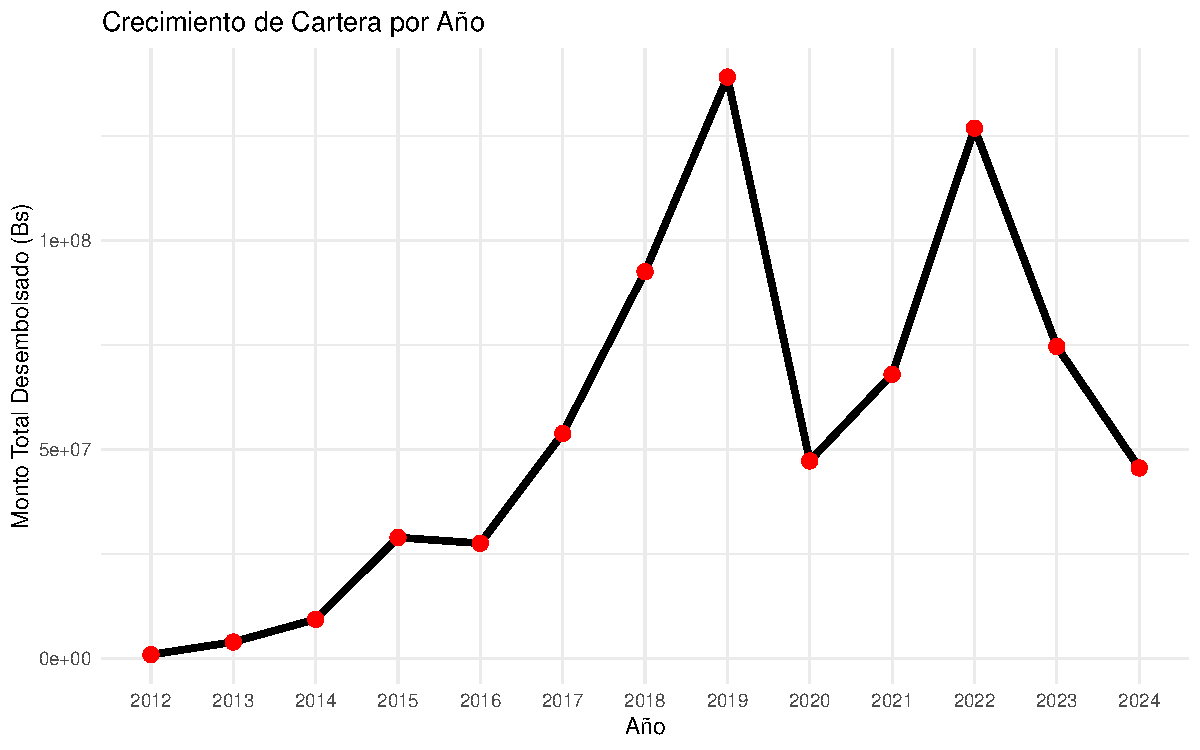
\includegraphics[width=0.9\linewidth]{Mineria2_files/figure-latex/graficos_ajustados-2} 

}

\caption{Crecimiento de Cartera por Año}\label{fig:graficos_ajustados-2}
\end{figure}

\textbf{Interpretacion (Figura 3)} El gráfico muestra la distribución de
clientes según su calificación crediticia dentro de CIDRE IFD. Se
observan las siguientes tendencias clave:

Predominio de clientes con calificación A

La mayoría de los clientes tienen una calificación A, superando los
6,500 casos.

Esto sugiere que CIDRE IFD mantiene una cartera con predominancia de
prestatarios confiables, lo que podría reflejar políticas crediticias
estrictas para minimizar el riesgo de mora.

Reducción drástica en clientes con calificación B y menores

La cantidad de clientes con calificación B es significativamente menor,
rondando los 500.

Las calificaciones C, D, E y F tienen valores marginales, indicando que
CIDRE IFD concede pocos préstamos a prestatarios de alto riesgo o que la
morosidad lleva a la exclusión progresiva de estos clientes.

Implicaciones para la gestión de riesgo crediticio

La alta concentración de clientes en categorías de bajo riesgo puede ser
positiva en términos de estabilidad financiera, pero podría limitar el
impacto de CIDRE IFD en la inclusión financiera de microempresas con
acceso restringido al crédito.

La baja representación en las calificaciones inferiores podría reflejar
una política conservadora de crédito, restringiendo el acceso a quienes
presentan mayor riesgo de mora.

Evaluar estrategias de seguimiento y reestructuración de cartera para
clientes con calificaciones intermedias (B y C) podría mejorar su
permanencia en el sistema financiero.

\textbf{Interpretacion (Figura 4)} El gráfico presenta la evolución del
Monto Total Desembolsado (Bs) en la cartera de CIDRE IFD desde 2012
hasta 2024. Se observan varias tendencias clave:

Crecimiento sostenido entre 2012 y 2019: Durante este período, el monto
desembolsado muestra un incremento significativo, lo que sugiere una
expansión en la colocación de créditos y una mayor confianza en el
sistema financiero.

Caída en 2020: Esta disminución puede estar vinculada a los efectos de
la pandemia del COVID-19, que impactó la economía y redujo la demanda de
crédito, especialmente en microempresas.

Recuperación parcial en 2021 y 2022: La cartera muestra una
recuperación, aunque no alcanza los niveles previos a la pandemia. Esto
puede reflejar una estabilización del mercado y el retorno progresivo de
la actividad económica.

Nueva contracción en 2023 y 2024: La tendencia descendente en estos años
indica posibles dificultades económicas, menor demanda de
financiamiento, o una política de crédito más cautelosa por parte de
CIDRE IFD.

\subsection{\texorpdfstring{10.
\textbf{Conclusiones:}}{10. Conclusiones:}}\label{conclusiones}

El análisis del comportamiento de la cartera de microcréditos de CIDRE
IFD entre 2022 y 2024 evidencia una tendencia de desaceleración
financiera impulsada por factores macroeconómicos y estructurales dentro
del país. La caída del PIB, el incremento de la informalidad laboral y
la escasez de divisas han generado condiciones de incertidumbre que
afectan la colocación y recuperación de créditos, particularmente en
sectores de microempresas y pequeños emprendedores.

El modelo de regresión confirma que la calificación crediticia es el
factor de mayor impacto en la probabilidad de mora, mostrando una
relación directa entre calificaciones bajas y el incumplimiento de
pagos. Asimismo, la tasa de interés ejerce un efecto significativo en la
acumulación de mora, lo que sugiere que un esquema de financiamiento con
tasas diferenciadas podría reducir el riesgo de incumplimiento. En
contraste, variables como edad, sexo y sector geográfico no presentan
una influencia relevante en la morosidad, lo que indica que el
comportamiento de pago está más ligado a factores financieros que
demográficos.

Los gráficos de evolución del monto desembolsado reflejan un crecimiento
sostenido hasta 2019, seguido de una contracción en 2020 debido a la
pandemia de COVID-19. Si bien CIDRE IFD mostró una recuperación parcial
en 2021 y 2022, la cartera volvió a disminuir en 2023 y 2024, reflejando
una crisis estructural que afecta la demanda de crédito y la estabilidad
financiera de los prestatarios.

\subsection{11. Bibliografía}\label{bibliografuxeda}

Fundación ABC Economía. (s.f.). La cartera de créditos y el microcrédito
en Bolivia (1era parte). Recuperado de:
\url{https://web.abceconomia.com/revista-n-95/la-cartera-de-creditos-y-el-microcredito-en-bolivia-1era-parte/}

Christen, R. P., \& Rhyne, E. (s.f.). Bolivia: Los más pobres, los más
atendidos. Microfinance.com. Recuperado de:
\url{https://microfinance.com/Castellano/Documentos/Bolivia_los_mas_Pobres.pdf}

Los Tiempos. (2024, abril 22). Microcréditos en Bolivia ya llegan al
31\% de la cartera de préstamos. Recuperado de:
\url{https://www.lostiempos.com/actualidad/economia/20240422/microcreditos-bolivia-ya-llegan-al-31-del-cartera-prestamos}

Money Bolivia. (s.f.). Microcréditos representan el 30\% de las
colocaciones del sistema financiero. Recuperado de:
\url{https://www.money.com.bo/ecofinanzas/microcreditos-representan-el-30-de-las-colocaciones-del-sistema-financiero/}

Fundación ARU. (s.f.). Evaluando el impacto de microcréditos en Bolivia:
Evidencia del Crédito Productivo Individual (BDP). Recuperado de:
\url{https://www.aru.org.bo/obs_desigualdad/doc/EvaluandoelImpactodeMicrocreditosenBolivia.EvidenciadelCr\%C3\%A9ditoProducitvoIndividual.BDP.pdf}

Fundación ARU. (2024, mayo). Empleo e ingresos de micro y pequeños
productores del área rural en Bolivia. Recuperado de:
\url{https://www.aru.org.bo/wp-content/uploads/2024/05/Bolivia_Empleo_e_ingresos_de_micro_y_pequenos_productores_del_area-1.pdf}

Fundación Milenio. (2024). Informe sobre la economía de Bolivia 2024
(N.º 46). Recuperado de:
\url{https://fundacion-milenio.org/informe-de-milenio-sobre-la-economia-de-bolivia-2024-n-46/}

FINRURAL. (s.f.). Sitio oficial de FINRURAL. Recuperado de:
\url{https://www.finrural.org.bo/}

CIDRE IFD. (s.f.). Nosotros -- CIDRE IFD. Recuperado de:
\url{https://cidre.org.bo/nosotros/}

\bibliographystyle{sageh}
\bibliography{bibfile.bib}


\end{document}
